\documentclass{beamer}
\usetheme{Warsaw}
\usecolortheme{default}
 
\title{\textsc{First Beamer Presentation}}
\subtitle{\LaTeX Beamer}
\author{Aidin Jalilzadeh}
\institute{UNNC}
\date{\today}
\begin{document}

\begin{frame}
\titlepage
\end{frame}

\begin{frame}\frametitle{Outline of Presentation}\label{outline}
\tableofcontents
\end{frame}

\section{Introduction}
\begin{frame}\frametitle{Introduction}\label{intro}
This is Intro
\begin{itemize}
\setbeamercovered{transparent}
\item<1-> Part A
\item <2-> Part B
\item <3-> Part C
\item <4-> Part D
\end{itemize}
\hyperlink{data}{\beamerskipbutton{Jump to Data}}
\end{frame}


\section{Terminology}
\begin{frame}\frametitle{Terminology}
\begin{description}
\item[AMS] American Mathematical Society
\item[PRC] Pepeoples Republic of China
\item[IBM] Integrated Buisness Machines
\end{description}
\end{frame}

\section{Main}

\begin{frame}\frametitle{Main}\label{main}
This is Main
\begin{columns}
\column{0.5\textwidth}<1->
jhsjsjjsjsjshvfjvfmnnbbmnb
jhgjjvdjsvjsavjvsaj,,bnnbmbmmb
shdjsjhsvbjvjdsh.nmnm,n,mn,
sdbjhsvjsvjsvbjhhbbbmmnmn 

\column{0.5\textwidth}<2->
\begin{figure}
\centering
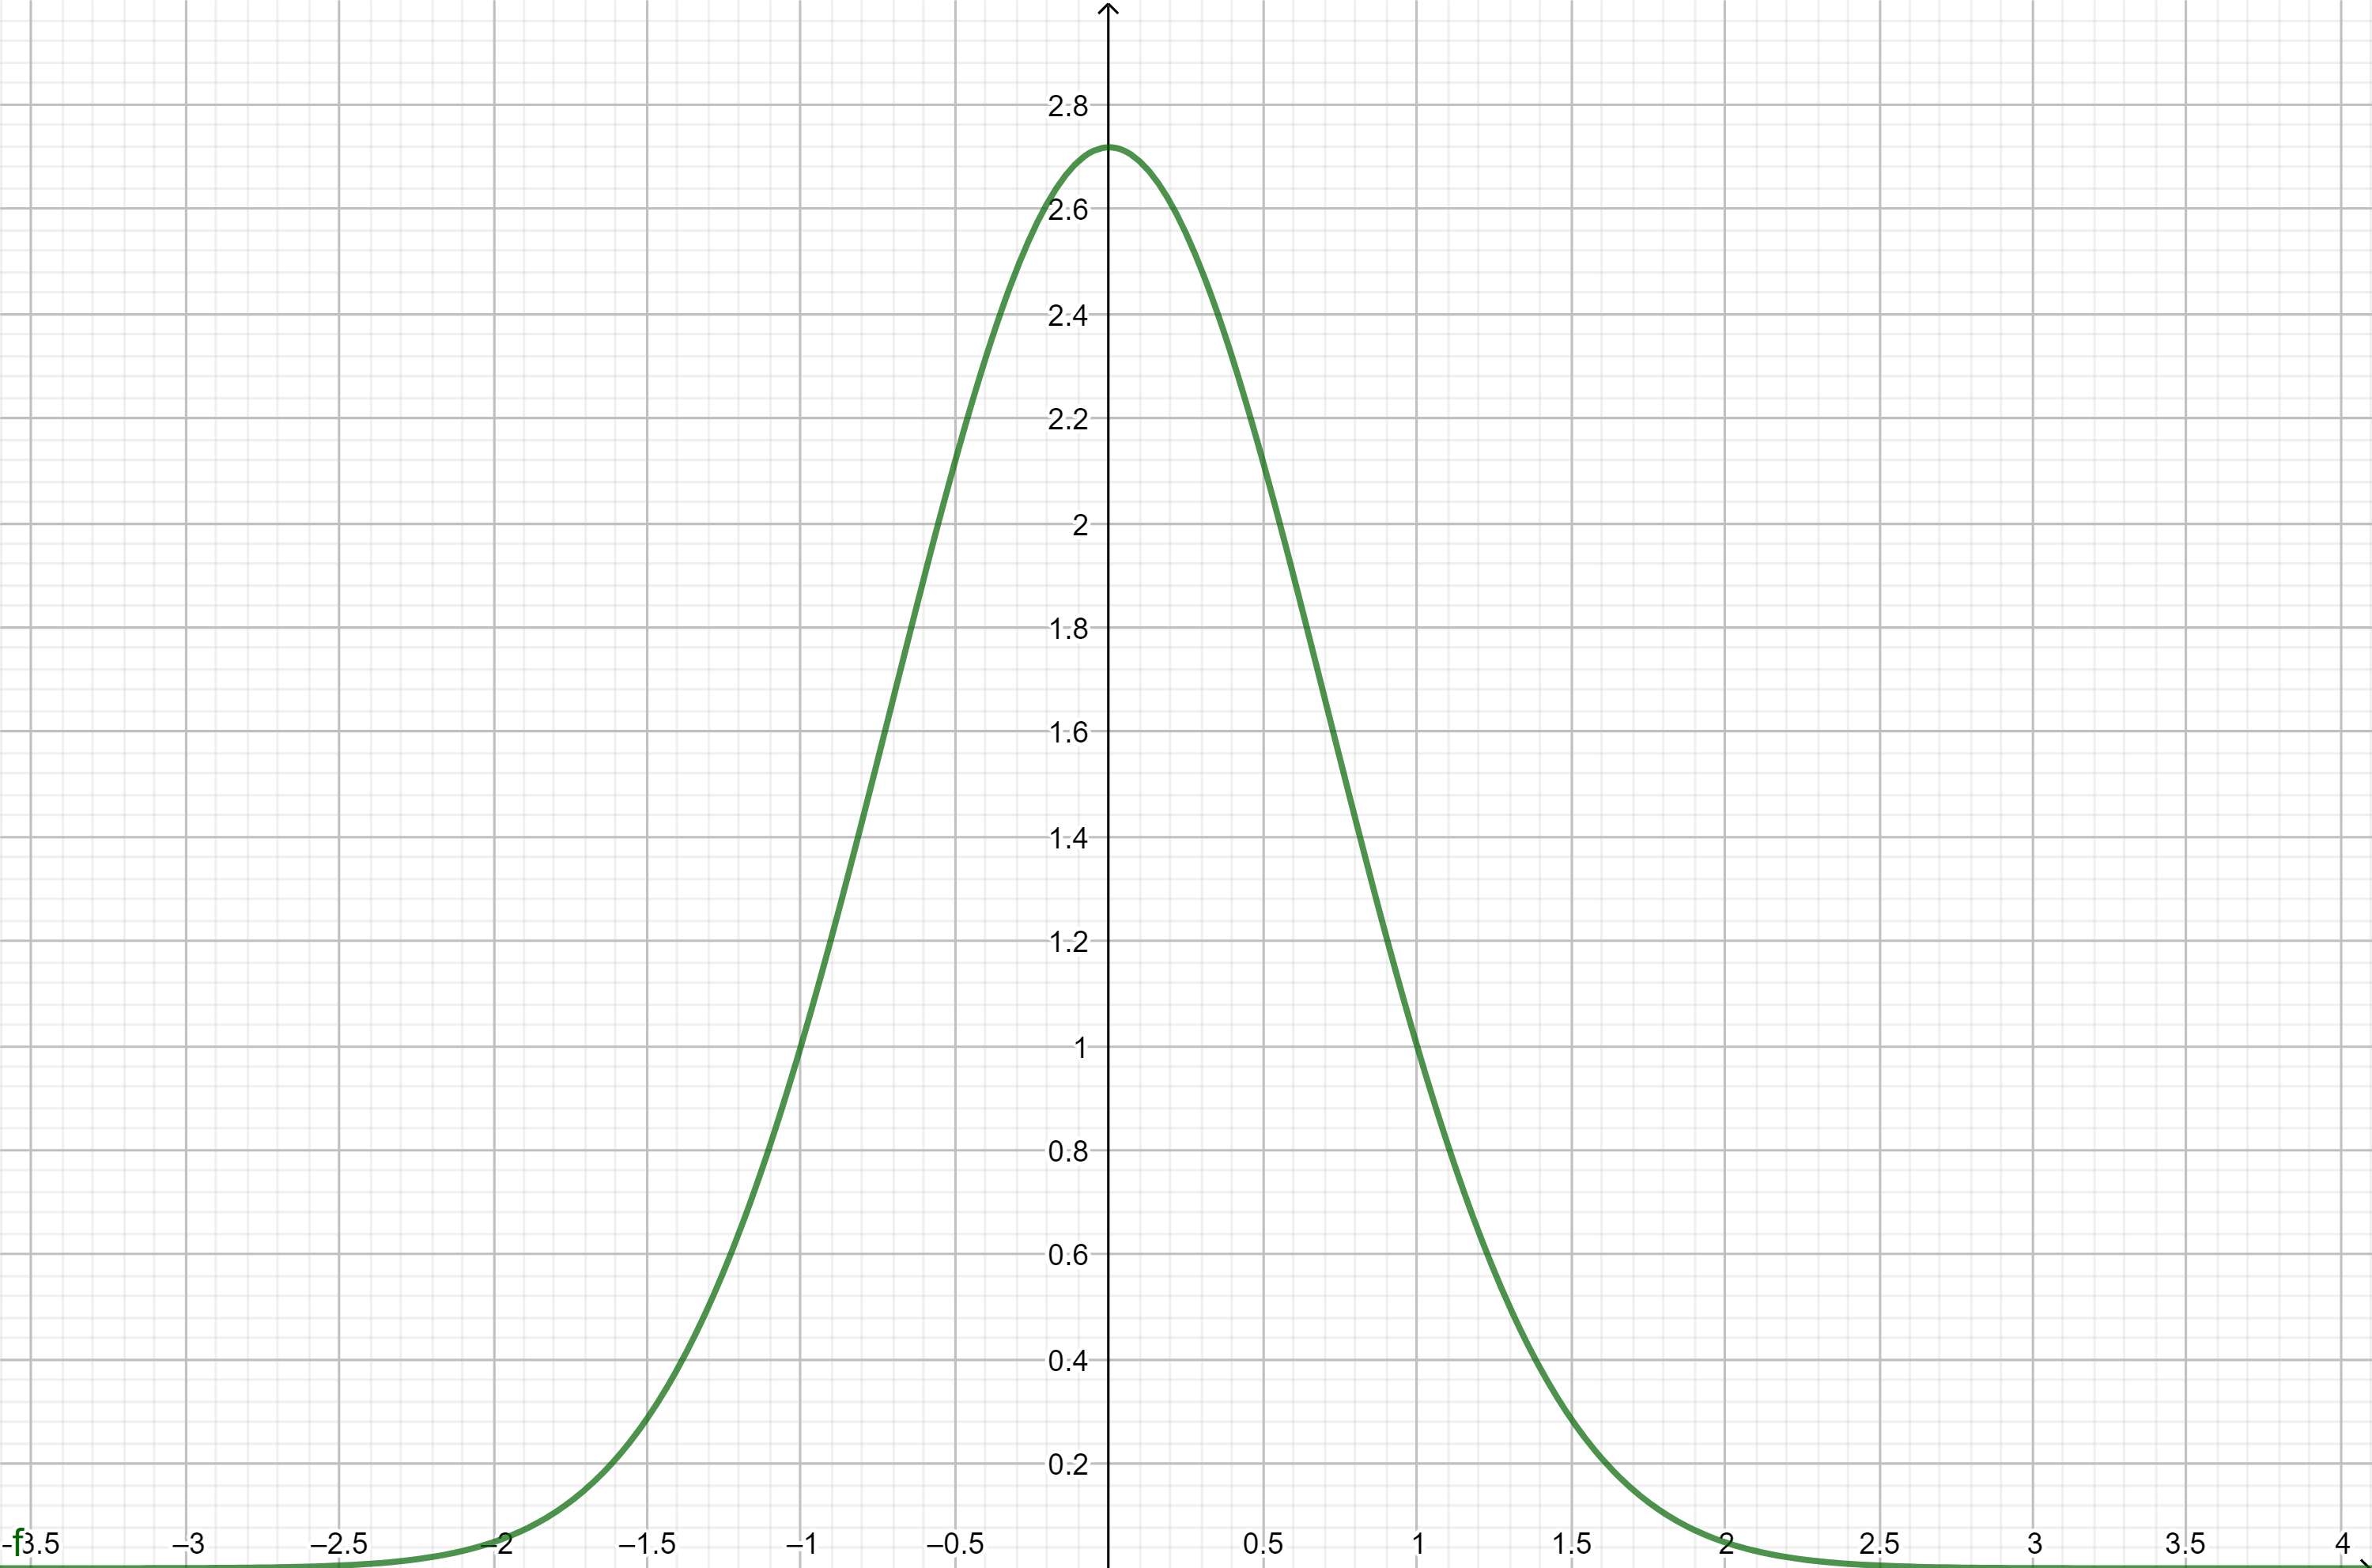
\includegraphics[scale=0.8]{plot0}
\caption{Primary Result}
\end{figure}
\end{columns}
\end{frame}

\begin{frame}\frametitle{Blocks}
\begin{block}{Block Title}<1->
This is a block ...
\end{block}

\begin{alertblock}{Alert Block}<2->
This is an alert block ...
\end{alertblock}

\begin{example}<3->
I am an example of good teacher !!
\end{example}

\begin{definition}<4->
Pythagoras: $x^2+y^2=z^2$
\end{definition}
\end{frame}

\section{Data}

\begin{frame}\frametitle{Data}\label{data}
This is Data
\begin{table}
\centering
\begin{tabular}{c|c|c}
A & 500 & 30 \\
\hline
B&400&70\\
\hline
C&800&10\\
\hline
\end{tabular}
\end{table}
\end{frame}
\section{Conclusion}

\begin{frame}\frametitle{Conclusion}
This is Conclusion
\begin{figure}
\centering
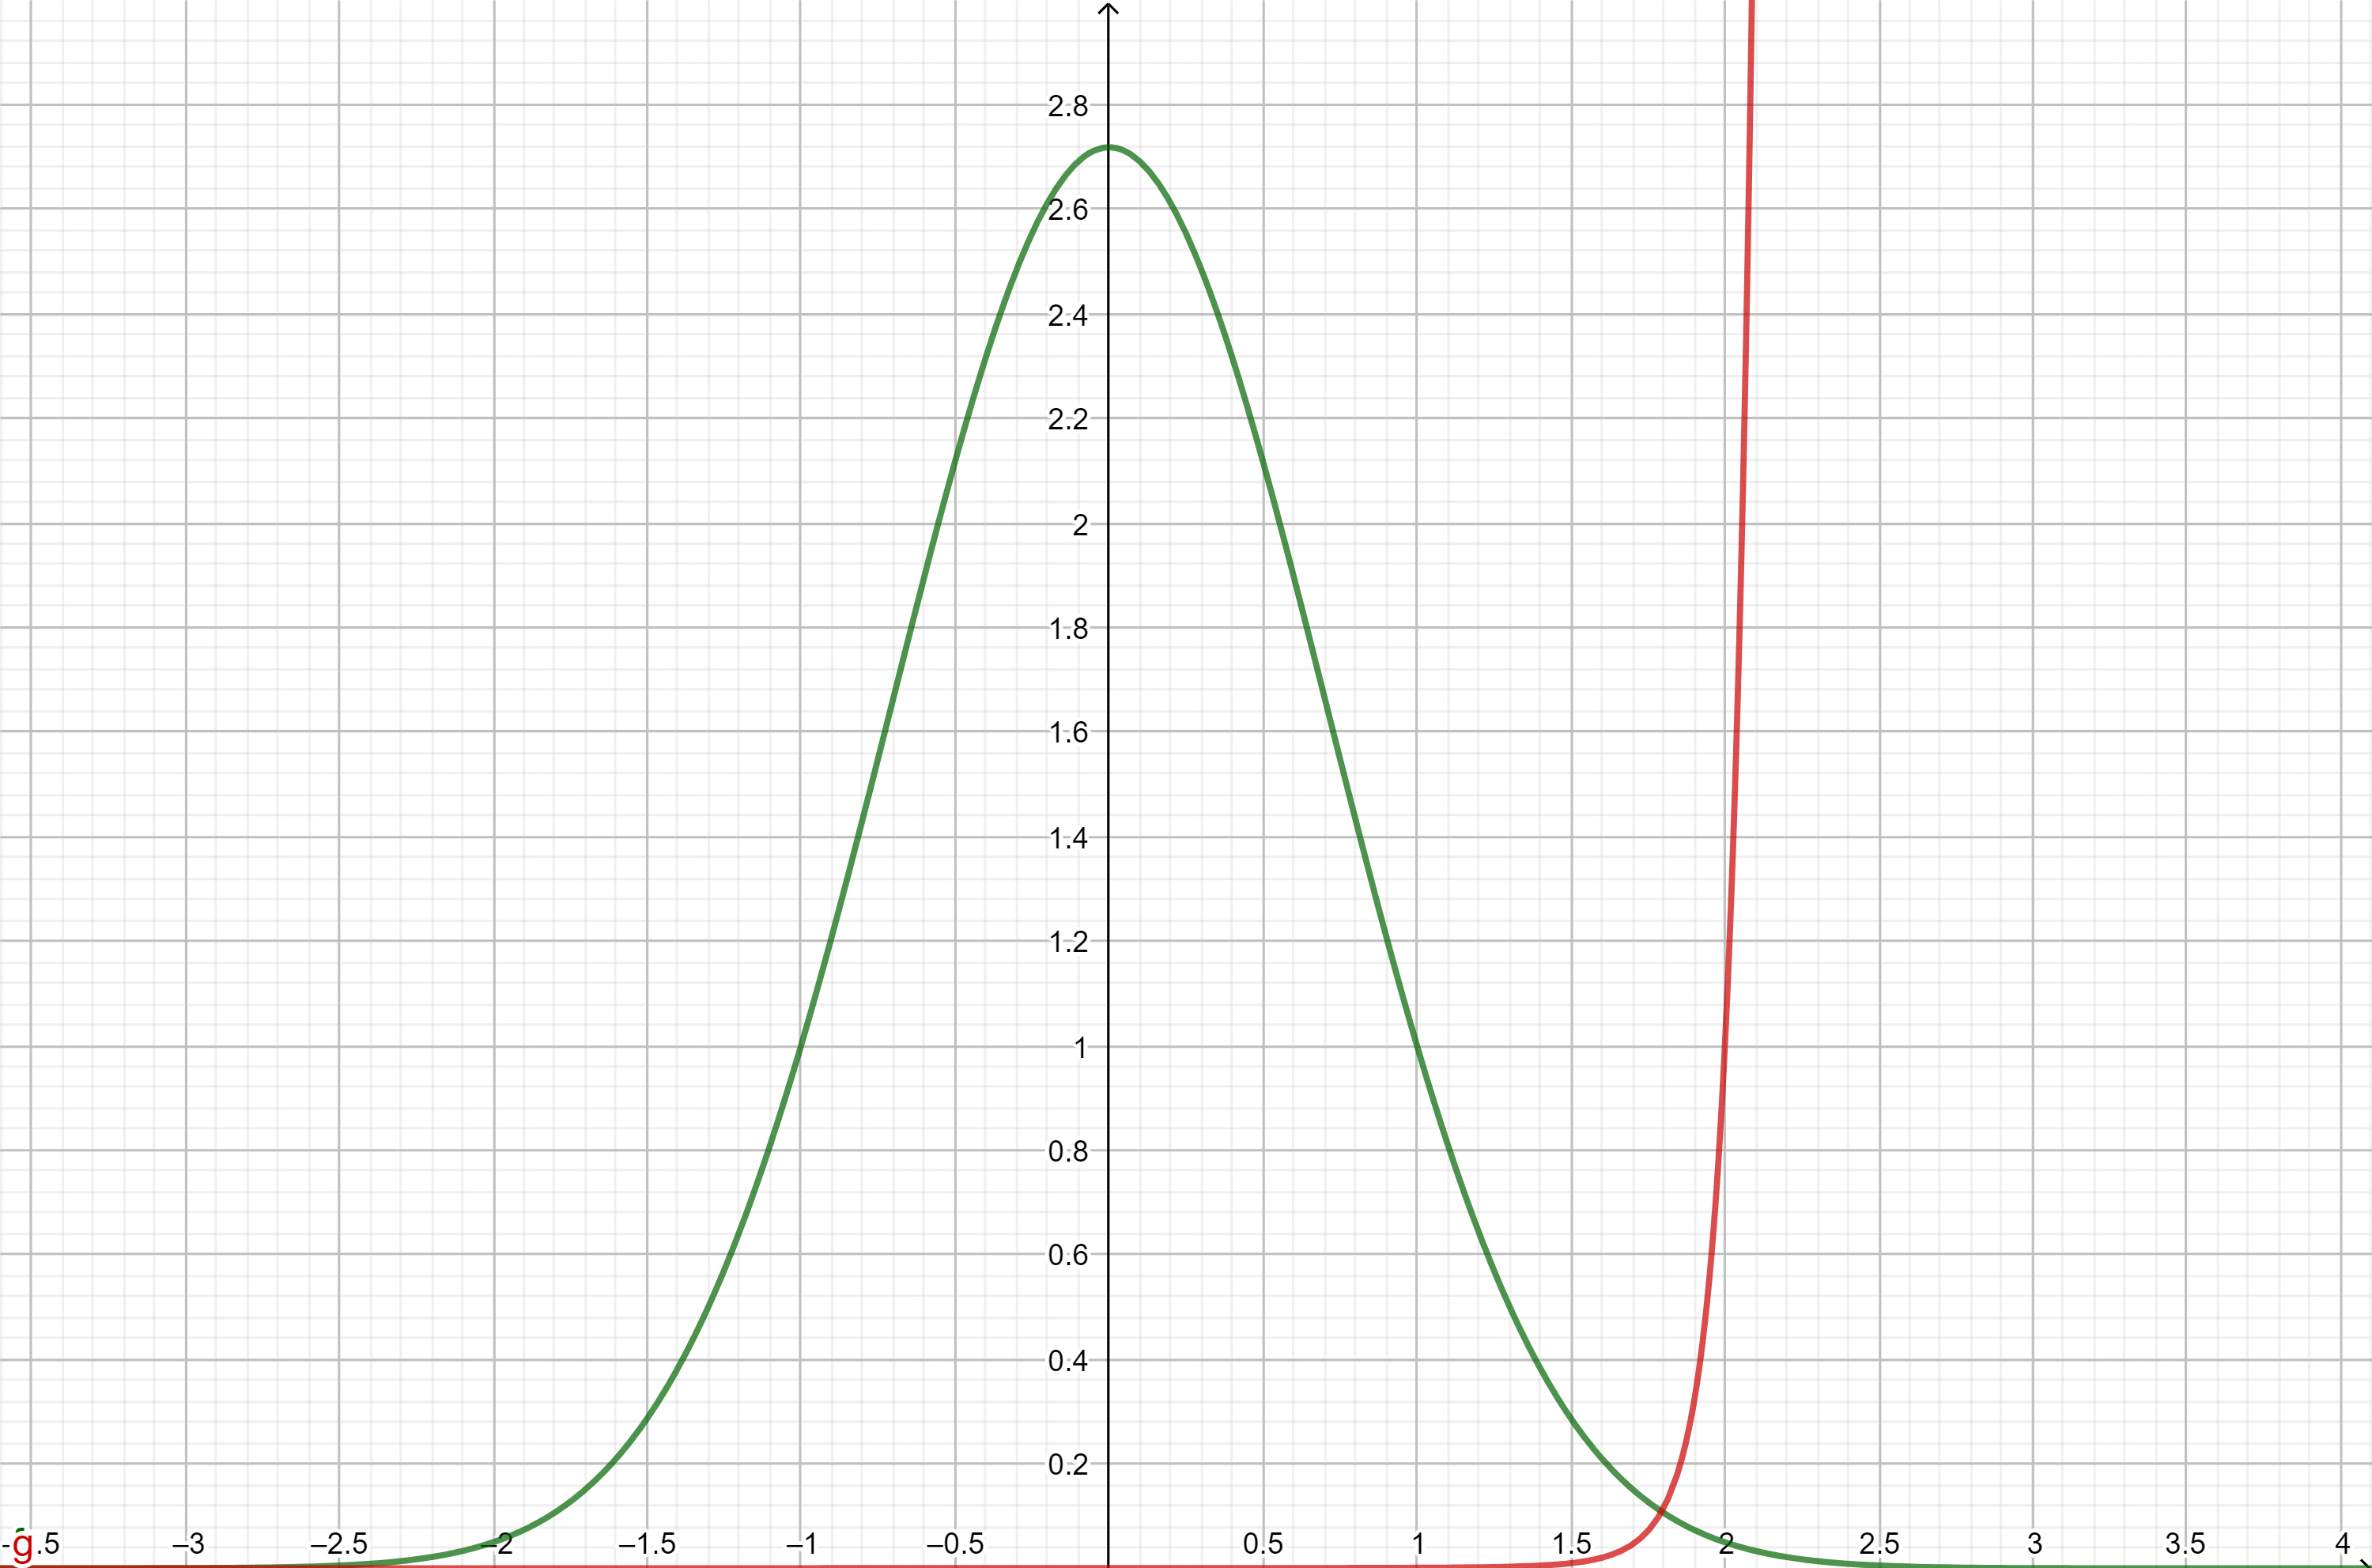
\includegraphics[width=9cm,height=5.5cm]{plot}
\caption{This is our result}
\end{figure}

\end{frame}

\begin{frame}\frametitle{Hyperlinks}
\hyperlink{outline}{\beamergotobutton{To Outline}}\\
\hyperlink{intro}{\beamergotobutton{To Introduction}}
\end{frame}

\end{document}